% Figure 1: Delta Accumulator Architecture
% For inclusion in main.tex via % Figure 1: Delta Accumulator Hardware
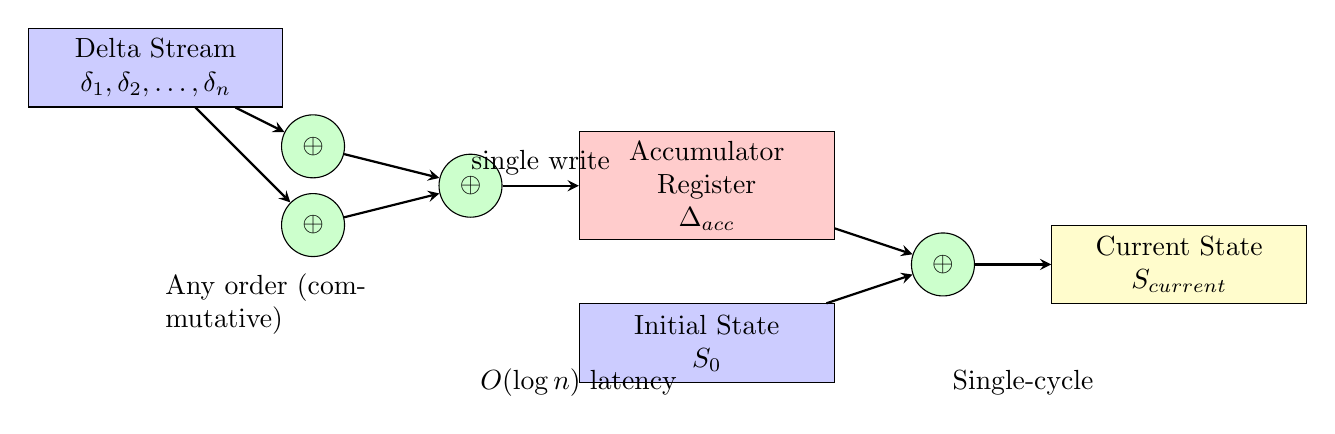
\begin{tikzpicture}[
    block/.style={rectangle, draw, fill=blue!20, text width=3cm, align=center, minimum height=1cm},
    xorgate/.style={circle, draw, fill=green!20, minimum size=0.8cm},
    arrow/.style={->, >=stealth, thick}
]

% Input deltas
\node[block] (input) at (0,4) {Delta Stream\\$\delta_1, \delta_2, \ldots, \delta_n$};

% XOR tree for parallel reduction
\node[xorgate] (xor1) at (2,3) {$\oplus$};
\node[xorgate] (xor2) at (2,2) {$\oplus$};
\node[xorgate] (xor3) at (4,2.5) {$\oplus$};

% Accumulator register
\node[block, fill=red!20] (acc) at (7,2.5) {Accumulator\\Register\\$\Delta_{\text{acc}}$};

% Initial state
\node[block] (init) at (7,0.5) {Initial State\\$S_0$};

% Final XOR for reconstruction
\node[xorgate] (final) at (10,1.5) {$\oplus$};

% Output
\node[block, fill=yellow!20] (output) at (13,1.5) {Current State\\$S_{\text{current}}$};

% Arrows
\draw[arrow] (input) -- (xor1);
\draw[arrow] (input) -- (xor2);
\draw[arrow] (xor1) -- (xor3);
\draw[arrow] (xor2) -- (xor3);
\draw[arrow] (xor3) -- node[above] {single write} (acc);
\draw[arrow] (acc) -- (final);
\draw[arrow] (init) -- (final);
\draw[arrow] (final) -- (output);

% Annotations
\node[anchor=west, text width=3cm] at (0,1) {Any order (commutative)};
\node[anchor=west, text width=3cm] at (4,0) {$O(\log n)$ latency};
\node[anchor=west, text width=3cm] at (10,0) {Single-cycle};

\end{tikzpicture}


\begin{tikzpicture}[
    delta/.style={draw, circle, minimum size=1cm, fill=blue!20},
    xor/.style={draw, circle, minimum size=0.8cm, fill=orange!30},
    state/.style={draw, rectangle, minimum width=1.5cm, minimum height=0.8cm, fill=green!20},
    arrow/.style={-{Stealth[length=3mm]}, thick}
]

% Input deltas
\node[delta] (d1) at (0, 3) {$\delta_1$};
\node[delta] (d2) at (0, 2) {$\delta_2$};
\node[delta] (d3) at (0, 1) {$\delta_3$};
\node[delta] (d4) at (0, 0) {$\delta_4$};
\node at (0, -0.8) {$\vdots$};
\node[delta] (dn) at (0, -1.8) {$\delta_n$};

% First level XOR
\node[xor] (x1) at (2.5, 2.5) {$\oplus$};
\node[xor] (x2) at (2.5, 0.5) {$\oplus$};

% Second level XOR
\node[xor] (x3) at (4.5, 1.5) {$\oplus$};

% Final accumulator output
\node[xor] (xacc) at (6.5, 0) {$\oplus$};

% Initial state
\node[state] (s0) at (6.5, -2) {$S_0$};

% Final state
\node[state] (sf) at (9, 0) {$S'$};

% Accumulated delta label
\node at (6.5, 1.5) {$\delta_{acc}$};

% Arrows
\draw[arrow] (d1) -- (x1);
\draw[arrow] (d2) -- (x1);
\draw[arrow] (d3) -- (x2);
\draw[arrow] (d4) -- (x2);

\draw[arrow] (x1) -- (x3);
\draw[arrow] (x2) -- (x3);

\draw[arrow] (x3) -- (xacc);
\draw[arrow] (s0) -- (xacc);
\draw[arrow] (xacc) -- (sf);

% Timing annotations
\draw[decorate, decoration={brace, amplitude=5pt, mirror}]
    (-0.5, -2.5) -- (5.5, -2.5) node[midway, below=5pt] {$O(\log n)$ parallel reduction};
\draw[decorate, decoration={brace, amplitude=5pt, mirror}]
    (6, -2.5) -- (9.5, -2.5) node[midway, below=5pt] {$O(1)$};

\end{tikzpicture}
